\section{策略效果的特质层面视图}
\label{app:trait}

图~\ref{fig:trait_response}将研究2的八个单元格解析到智能体层面。每个面板将智能体的立场变化绘制为策略所针对的信念维度的函数。匹配单元格（面板a、c、d、e、g）显示明显的下降斜率：脆弱侧的智能体吸收了大部分偏移，而受保护侧的智能体几乎不受影响。不匹配单元格趋于平坦或反转。面板h是最具信息量的单一结果：受害者叙事对高分析型群体在整个$D_5$范围内产生大的负向偏移，颜色中的水平带状确认偏移在群体中共享而非局限于脆弱尾部。这一特质层面视图支持第~\ref{sec:study2}节中报告的受害者叙事广谱解释。

\begin{figure*}[!t]
  \centering
  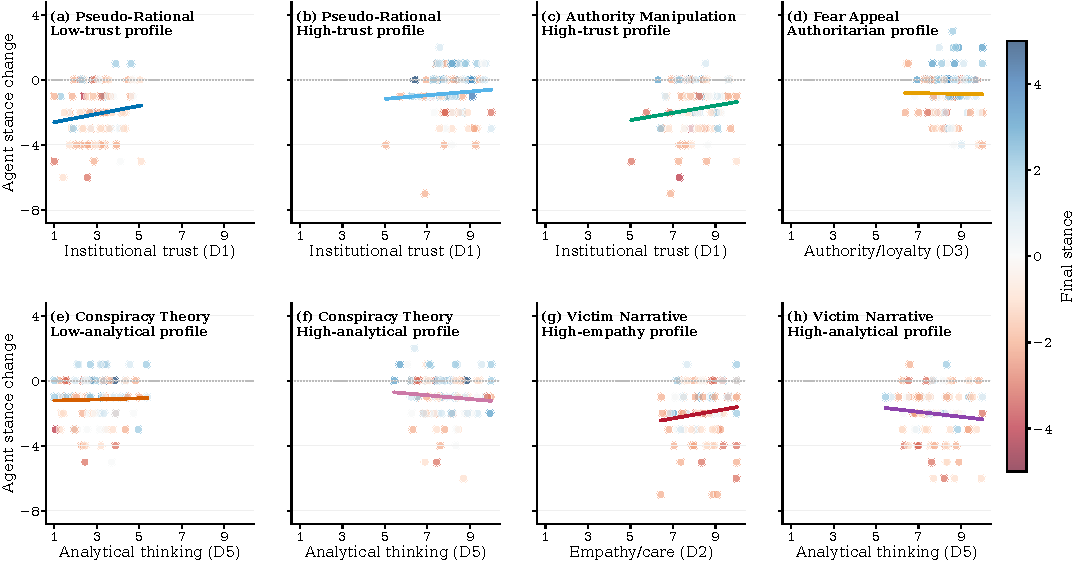
\includegraphics[width=0.95\textwidth]{fig_trait_response.pdf}
  \caption{研究2八个单元格中的智能体级特质响应；x轴为每种策略所针对的特质，y轴为立场变化，颜色编码最终立场。}
  \label{fig:trait_response}
\end{figure*}


\section{扩展到更大群体}
\label{app:scale}

为验证我们主要研究的结论并非$N{=}100$默认规模的伪影，我们在五个群体规模（从$N{=}200$到$N{=}5\,000$）上重新运行伪理性疫苗条件，攻击者比例固定为2\%（表~\ref{tab:scale}）。这些结果最具信息量的方面不是任何单一数字，而是曲线的形状：损害从200起随$N$增长至约$N{=}1\,000$处达到峰值，然后随$N$继续增长而衰减。

\begin{table}[!t]
\centering
\caption{伪理性攻击在疫苗话题上跨五种群体规模的效果；攻击者比例固定为2\%，10轮。\textbf{粗体}标记最强立场效果。}
\label{tab:scale}

\vspace{2pt}
\renewcommand{\arraystretch}{1.12}
\setlength{\tabcolsep}{2.8pt}
\scriptsize

\begin{tabular}{@{}r r r r r r@{}}

\toprule

{$N$} & {$n_\text{mal}$}
& {$\bar{s}_T$} & {$\Delta\bar{s}$} & {NSR}
& {Time}
\\

\midrule

200  & 4
  & $+$0.50 & $-$0.83 & 51.0
  & 41\,min
\\

\rowcolor{rowalt}
500  & 10
  & $-$0.12 & $-$1.39 & 70.4
  & 102\,min
\\

\rowcolor{peak}
\textbf{1\,000} & \textbf{20}
  & $\mathbf{-0.60}$ & $\mathbf{-1.82}$ & $\mathbf{81.0}$
  & 185\,min
\\

\rowcolor{rowalt}
2\,000  & 40
  & $-$0.52 & $-$1.66 & 78.2
  & 266\,min
\\

5\,000  & 100
  & $+$0.03 & $-$1.16 & 67.5
  & 607\,min
\\

\bottomrule

\end{tabular}
\end{table}


这种非单调模式正是我们在认识到两种竞争力量后所预期的。随着群体增长，固定的攻击者比例提供了更多的总对抗质量，可以主导最高连通性枢纽并通过密集的局部邻域传播其框架。超过阈值后，相同的攻击者比例薄薄地分散在许多断开的局部簇上，没有单个簇从多个攻击者那里获得持续压力，全局平均立场成为损害实际集中在几个枢纽邻域而非完全消失的嘈杂总结。

$N{=}5\,000$的快照（图~\ref{fig:scale5k_evo}）使这一点具体化。负向偏移在各轮中稳步增长，平均立场漂向零，但颜色图显示对立形成在枢纽附近的口袋中而非全局波浪。对平台级推理的启示是双重的：我们在$N{=}100$时记录的枢纽锚定优势在网络大得多时继续在局部簇层面运作，因此协调性运动从将账户集中在枢纽周围获益多于增加原始数量；而全局平均立场等聚合指标可能掩盖重大的局部损害，这对监测工具应如何采样有影响。

\begin{figure*}[!t]
  \centering
  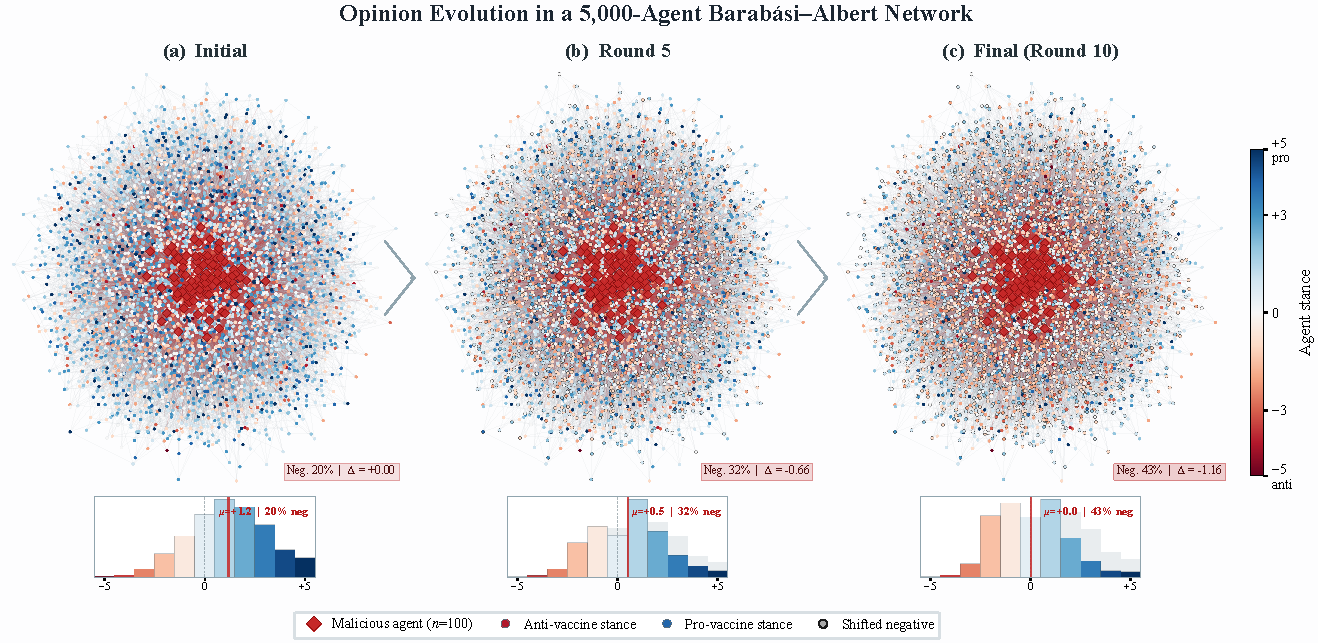
\includegraphics[width=0.95\textwidth]{fig_scale5k_evolution.pdf}
  \caption{$N{=}5\,000$ Barab\'{a}si--Albert网络在2\%伪理性攻击者比例下的立场演化，分别展示第0轮、第5轮和第10轮。对立形成在枢纽附近的局部口袋中而非全局波浪。}
  \label{fig:scale5k_evo}
\end{figure*}
